%----------------------------------------------------------------------------------------
%   PACKAGES AND OTHER DOCUMENT CONFIGURATIONS
%----------------------------------------------------------------------------------------

\documentclass[11pt]{article}

\usepackage[english]{babel}
\usepackage[utf8x]{inputenc}
\usepackage{amsmath}
\usepackage{graphicx}
\usepackage{csquotes}
\usepackage{fancyvrb}
\usepackage[a4paper, total={6in, 8in}]{geometry}
\usepackage[colorinlistoftodos]{todonotes}

%----------------------------------------------------------------------------------------
%   HEADING
%----------------------------------------------------------------------------------------

\newcommand{\BigO}[1]{\ensuremath{\operatorname{O}\left(#1\right)}}

\title{\textsc{Software Engineering}\\Main Coursework II}
\author{Lawrence Jones \{lmj112\} \  Alice Sibold \{as4712\} \\
        Joshua Coutinho \{jrc12\}}

\date{}
\begin{document}
\maketitle

%----------------------------------------------------------------------------------------
%   BODY
%----------------------------------------------------------------------------------------

GoCardless, established in 2011, is a FinTech start-up based in Angel, London.
Their main product is an API that instruments Direct-Debit payment networks to
pull money between bank accounts, making GoCardless a great case study for
modern technological practices in start-ups.

In contrast, Amazon is the largest internet retailer in the United States with
an internationally recognised brand. Launched in 1994, Amazon stands as one of
the greatest successes of the internet, weathering the dot-com collapse and many
competitors. Amazon also supports one of the largest micro-service architectures
after hitting a barrier in 2001, when its C++ Obidos monolith would take over a
weekend to compile.

This article compares the software development lifecycle (SDLC) between two
companies with disparate operational scales, company history and ethos.
Techniques that work well for one company can become severe hindrances when
scaled, and it will be interesting to see which survive over the course of that
transformation.

\section{Conception}


Developers at GC tackle new features with a `kick-off' meeting, consisting of
the core development team and any other essentially involved people from around
the company. The aim is to discuss the critical path of the feature, describing
the experience for the standard user.  Any issues can be raised while the people
with domain knowledge are present, allowing the plan to adjust to immediate
feedback before any real work is done.

The team of developers then produces a `scoping document'
(Figure~\ref{fig:scoping}) in a collaborative environment (e.g. Google Docs),
detailing their implementation plan, capturing the research around the feature;
directly involved individuals are notified and it is accessible to everyone.

\begin{figure}
\centering
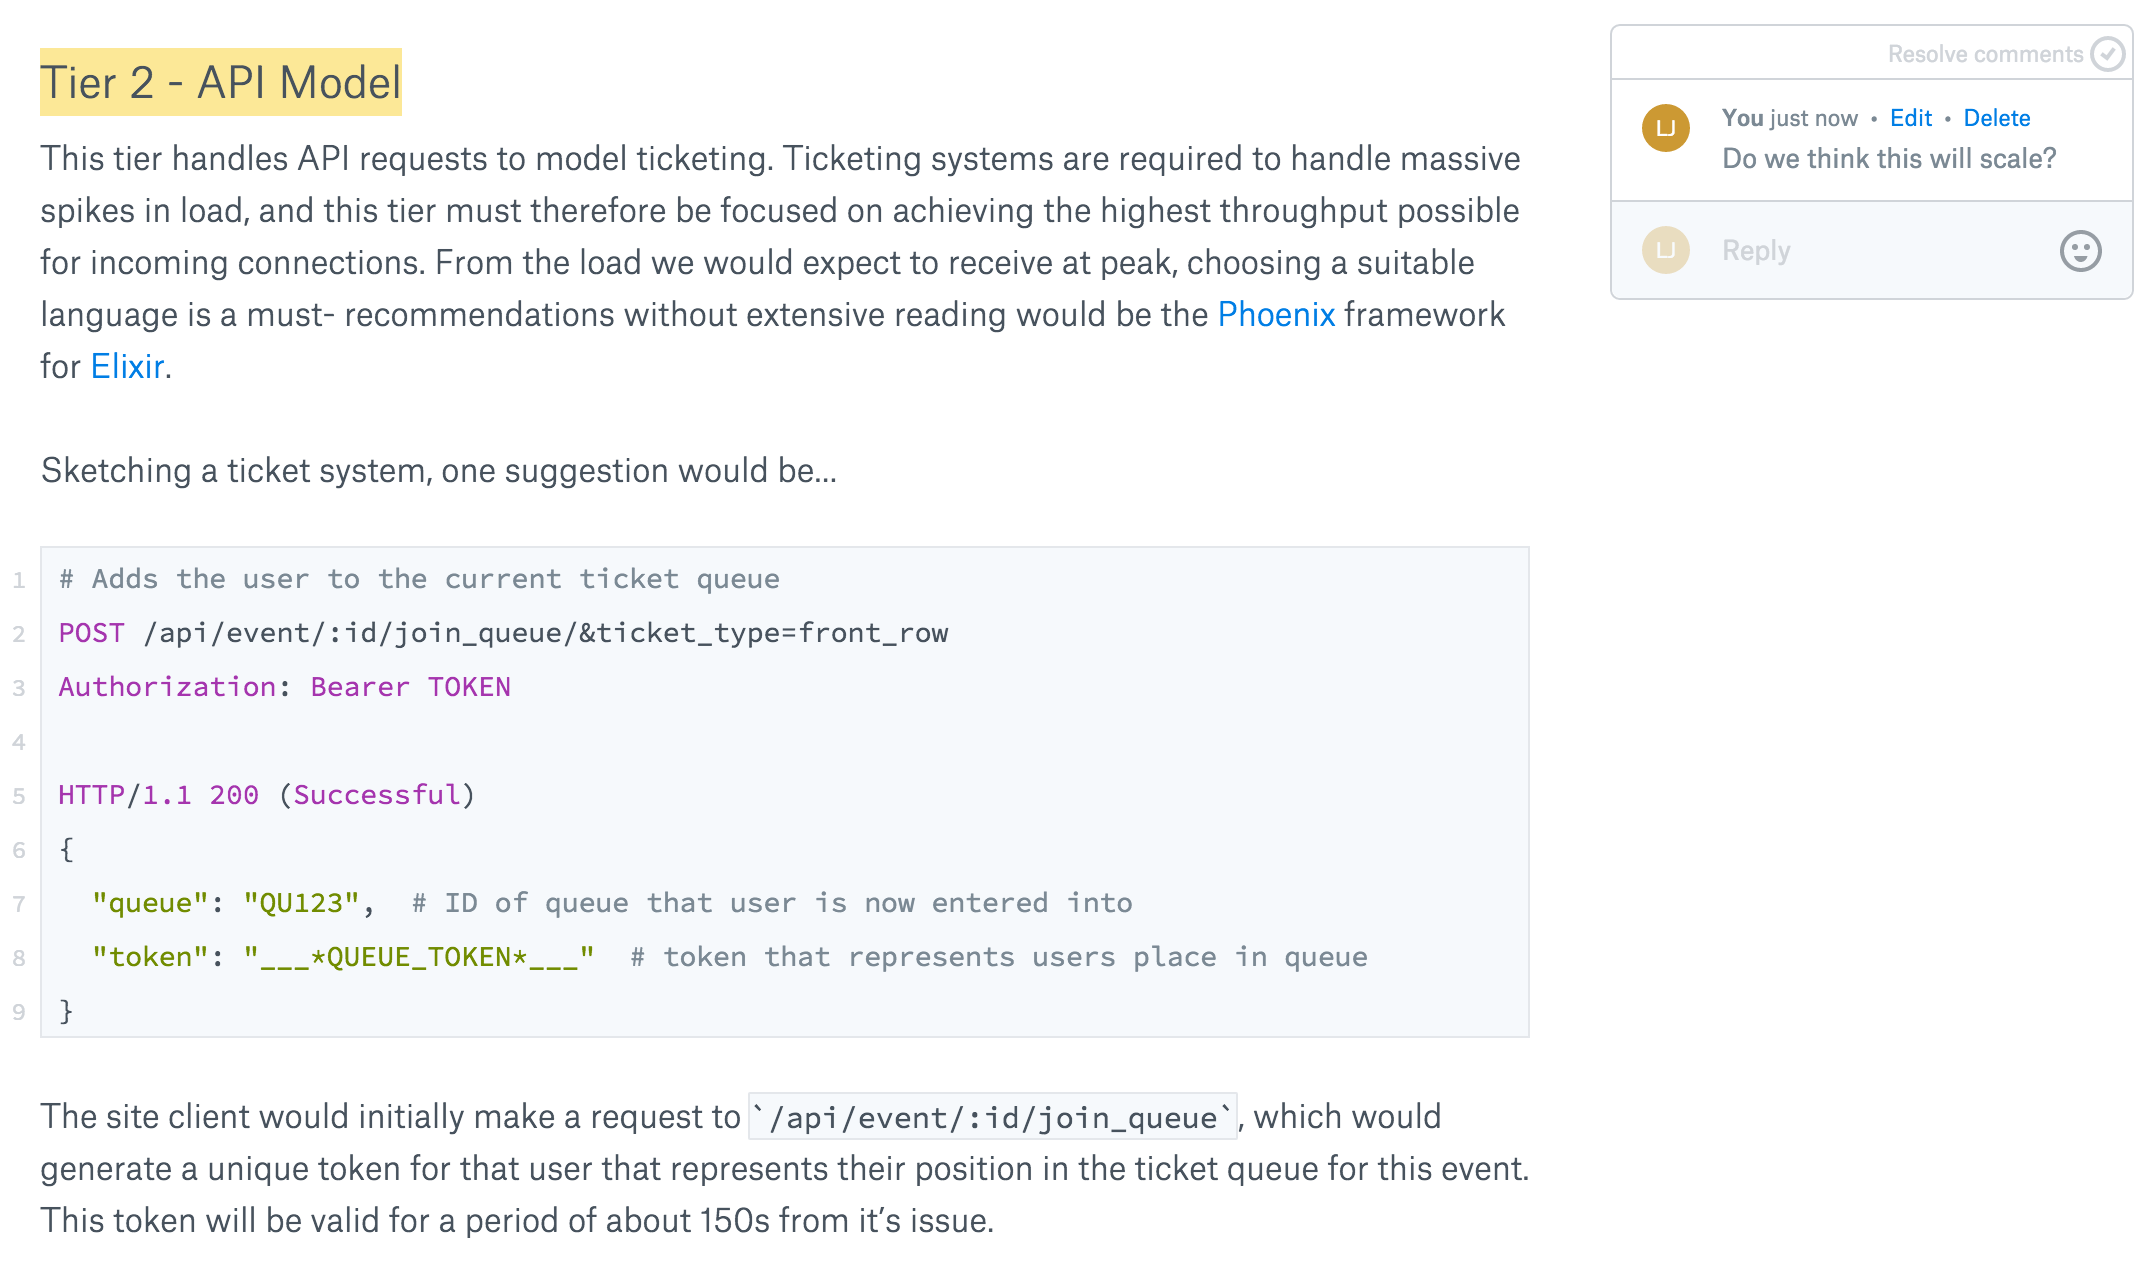
\includegraphics[width=0.9\textwidth]{lib/res/scoping.png}
\caption{\label{fig:scoping}\textit{Example scoping document- mix of technical with
free-form content}}
\end{figure}

Working with such visibility enables operational benefits. Foremost, the
solutions almost always address actual requirements. Having others who
understand the problem at hand during the design process means misunderstandings
are stemmed early, with minimal cost~\cite{costOfChangeEssay}.

Secondly, opening this document to the company increases awareness of what the
development team are working on. For non-developers, this translates into an
understanding of how a large part of the company are spending their time, and
how that work contributes to the overall company's goal. A key component of any
high functioning team is accountability within the
sub-teams~\cite{fiveDysfunctions}, and this only comes when teams have an
understanding of what others are working on.

For developers, this increased visibility means a direct reduction in the
projects bus, or truck factor~\cite{truckFactor}. When other developers can
share in the design process they learn crucial information that will help them
troubleshoot code when problems arise in the future. Beyond this, any developers
who conceive an alternative approach or predict problems with the design have a
clear forum for discussion.

At Amazon new employees are told business proposals must be grounded in solid
research; who makes them is irrelevant. Teams communicate preferably through
whitepapers, a type of concise free-form summary. This forces the presenter to
compact their research into something easily digestible.

Amazon's whitepapers are similar to GoCardless's scoping document, and have the
same aim although it lacks the collaboration of online tools. They follow a top
down structure~\cite{reportingAndWriting}, where they explore the topic at an
increasing level of detail. This aids inter-team communication and allows at
least part of the documents to be readable, while still providing technical
details.

The effect of this is profound. It forces the developer to identify assumptions
behind each stage of the project plan. By walking through each implementation
step the developer questions what the task will consist of, leading to to an
improvement in estimation accuracy and fewer implementation surprises.

The Agile Manifesto~\cite{agileManifesto} states `[We value] working software
over comprehensive documentation' which has impacted the perceived value of
technical documents to many modern developers. We argue that a whitepaper does
not constitute `comprehensive' documentation, and its advantages are as relevant
now as when Joel Spolsky wrote his article `Painless Functional Specifications -
Why Bother?' in 2000.

Joel argues that `specs' aid in funnelling out inaccurate assumptions developers
may have about the product, preventing inaccurate code. We tackle this problem
at the earliest stage, before our software resembles `a compromise between the
initial, wrong design and the ideal design'. This focus also lends itself to
forcing decisions on the hardest problems, those which are often put off until
the last moment, despite being the issues most likely to cause a software
project to fail.

Technical documents can be considered heavyweight tools, long since replaced in
software-engineering. We counter that they remain a valuable tool aiding
investigation into a problem, as well as an anchor for inter-team communication.
That Amazon and GoCardless use such tools when both are fast-moving environments
striving for optimal efficiency suggest that technical writing may be less
restrictive that it at first seems.

\section{Testing \& Continuous Delivery}

Amazon recently released tools that allow developers to automate code deployment
via the AWS console. AWS CodeDeploy and CodePipeline are continuous delivery
instruments, and bring advanced deployment tools within reach of your standard
developer.

\begin{figure}
\centering
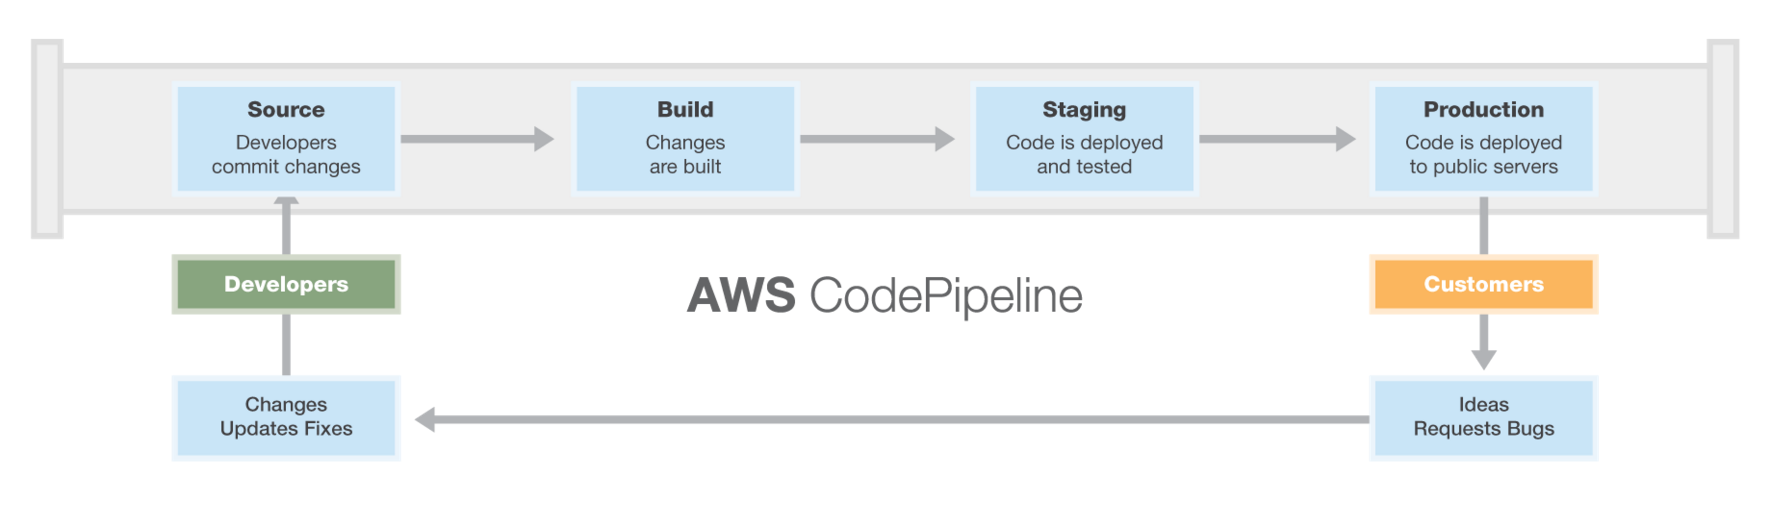
\includegraphics[width=0.8\textwidth]{lib/res/code_pipeline.png}
\caption{\label{fig:scoping}\textit{Diagram from Amazon webpage on
CodePipeline}}
\end{figure}

While this is the first time tools like this have been offered by Amazon
commercially, they have existed as internal tools for many years. Amazon's
platform is built on top of micro-services; upto 150 services are invoked per
page render. As one of the first companies to embrace micro-services, Amazon
tackled novel growing pains as they built out their architecture from the old
monolith.

The most significant of was how much developer time was sunk into deployments.
Now Amazon was split into may services, each team had their own deployment
strategy. When deployment is \texttt{ssh}'ing into a single box then this isn't
an issue, but Amazon was deploying to fleets of hundreds of servers with
zero-downtime requirements. No unified tool-chain for deployments cost meant
each team re-invented the wheel, producing bespoke deployment processes for
their service. Werner Vogels describes the problem\dots

\begin{displayquote}

  Each team took on full ownership of the development and operation of a single
  service\dots teams were able to quickly produce new features, but their deployment
  process soon became a bottleneck. Manual deployment steps slowed down releases
  and introduced bugs caused by human error. Many teams started to fully
  automate their deployments to fix this, but that was not as simple as it first
  appeared.

  \textit{The Story of Apollo - Amazon's Deployment Engine~\cite{theStoryOfApollo}}

\end{displayquote}

Amazon's internal deployment platform, Apollo, was built to solve this problem.
`The Deployment Production Line'~\cite{deploymentProductionLine} defines
qualities of good deployment systems, and Apollo satisfied many of these.

The first is automating deployments. Apollo offered full, intelligent automated
deployment of services, across a fleet of AWS servers. Once configured, Apollo
could deploy code to any required environment, spinning up servers to match the
application's scaling profile, and configuration changes could be made on the
fly without no service downtime. This was far beyond the custom shell scripts
teams had written. Apollo benefited from a dedicated team working full time on
features, while integrating the tool into Amazon's infrastructure, immediately
reducing the amount of time developers spent debugging their deployments.

Humble states that a deployment tool chain must ensure the same artifacts are
deployed to every environment. Each service at Amazon depends on hundreds of
others, and so building against the correct version-set is essential for
reliability. Amazon solves this problem with another tool, called Brazil, which
is used as the bootstrapper whenever running an Amazon service.

Each service (synonymous here with package) has its own Brazil config file,
containing a mapping of each dependency to version. Brazil can be used to pull
down and install a service's dependencies but crucially, Brazil can lockdown a
machine to use only those packages installed from the Brazil config.  Each
service is invoked through a shim, \texttt{brazil-bootstrap}, which hijacks the
system path to point only to the dependencies installed from the config file.
All services are built and deployed using Brazil, ensuring that each environment
benefits from repeatable builds that rely on exactly the same dependency
versions.

This method of enforcing good practise on developers is typical of Amazon's
working environment. Having thousands of developers working on Amazon services
precludes simply sending a memo about a new development process. The power of
linking every developer into a unified deployment tool (such as Apollo) is that
company-wide standards can be baked into every teams process.

One of the greatest examples of how Amazon use this power is to enforce a best
practise that very few in the industry have managed to adhere to- unit tests
should run in isolation, without hitting any external resources. Clean
Code~\cite{cleanCode} states five qualities of good unit tests, two of which
demand this property\dots

\begin{displayquote}

  \textbf{Fast}: Tests should be fast. The should run quickly. \\
  \textbf{Repeatable}: Tests should be repeatable in any environment. \\

  \textit{Robert C. Martin. `Clean Code: A Handbook of Agile Software
  Craftsmanship.'}

\end{displayquote}

When unit tests need to run fast, they cannot rely upon external components that
may take many seconds to generate responses. Dependence on external services
violates repeatability - test output is tied to that service its returned value.

Amazon ensures that all unit tests are written in this way by locking down the
boxes in the unit test pipeline stage, with firewalls that block any network
attempt out, or back into the host, removing the possibility of communicating
with a locally hosted database for example. Consequently, tests run in under 10m
including setup and teardown, without relying on any specialised hardware or
parallelisation. This minimises the cost per build while preserving rapid
feedback to developers.

GoCardless' process is more flexible, encouraged by Ruby on Rails. Rails uses a
framework called \texttt{ActiveRecord}~\cite{activeRecord} as a database ORM,
abstracting away from the underlying database to provide an interface that can
be called from Ruby code. While key to Rails development, using
\texttt{ActiveRecord} means your code implicitly relies upon an active database
connection.

Unit tests that hit \texttt{ActiveRecord} now break the `repeatable' quality
that states tests should run in any environment. Standard practise for writing
Rails tests will use \texttt{gems} such as
\texttt{FactoryGirl}~\cite{factoryGirl} to create mock database records before
each test run. This practise can be very slow, and without due care test suite
running time can balloon. Writing tests in this fashion sacrifices some speed
and resilience of idiomatic unit tests, but has its benefits\dots

\begin{displayquote}

  Writing semi-integration instead of unit tests is just easier than the
  alternative. When the code under test relies on \texttt{ActiveRecord} and some
  features like database transactions, it's much quicker to not put the work
  into building reusable mocks and decomposing things so they can be tested
  without hitting the database.

  The trade off is very cheap when the system is small- you don't have many
  tests so even if each one is super-slow it doesn't matter. The problem appears
  when the system grows, as the cost increases exponentially and you end up with
  $>5m$ builds, which can become a waste of developer time. \\

  \textit{Isaac Seymour - Backend developer at GoCardless}

\end{displayquote}

So if this becomes a such a problem, why are GoCardless willing to suffer it?
\texttt{payments-service}, the core system behind the GoCardless API, is a Rails
app consisting of over 150k lines of Ruby code. Surely this problem should have
crossed the line at which point build times become prohibitively expensive?

Unfortunately, \texttt{payments-service} has a few characteristics that make it
more difficult than your standard Rails app to test in isolation. The first is
due to defensive programming- working with payments means protecting against
software errors that can cause bad accounting, including race conditions.
GoCardless engineers decided early on to rely on the database layer to provide
atomicity guarantees, and so code often relies on \texttt{ActiveRecord} passing
up database exceptions, such as constraint violations.

Mocking how \texttt{ActiveRecord} handles the underlying database in a unit test
is infeasible. Test code becomes a game of how well the developer knows
\texttt{ActiveRecord} internals, and is inherently fragile. Mocking constraint
violations can expose the risk that unit tests will pass (simulating the
constraint being violated) without the constraint ever being encoded into the
database.

When your app moves millions of pounds daily, even that minimal risk cannot be
tolerated. Zach Holman states\dots

\begin{displayquote}

  `We can make good tests run fast but we can't make fast tests be good.'

  So start with a good foundation: have good tests. Don't skimp out on this,
  because it impacts everything else down the line. \\

  \textit{Zach Holman - How to Deploy Software~\cite{howToDeploySoftware}}

\end{displayquote}

GoCardless opted to write good tests over the faster, more brittle kind they
felt were an inevitability had they mocked out the database. But Zach suggests
we can push the envelope on how far we can run with these tests, and indeed
GoCardless do just that. By tuning PostgreSQL for maximal testing performance,
you can immediately reduce the running time of database heavy tests.

While useful, these optimisations only go so far. Zach says
~\cite{howToDeploySoftware} that test suites should run in the range of 5-10m,
and throwing more hardware at the problem can be a viable solution. The cost of
additional infrastructure can be justified in the time it saves for developers
when checking in a new change, and GoCardless tackles this problem by sharding
unit tests on their CI provider. This brings test suite running time down to 10m
for \texttt{payments-service}, as can be seen in Figure~\ref{fig:circle}.

\begin{figure}
\centering
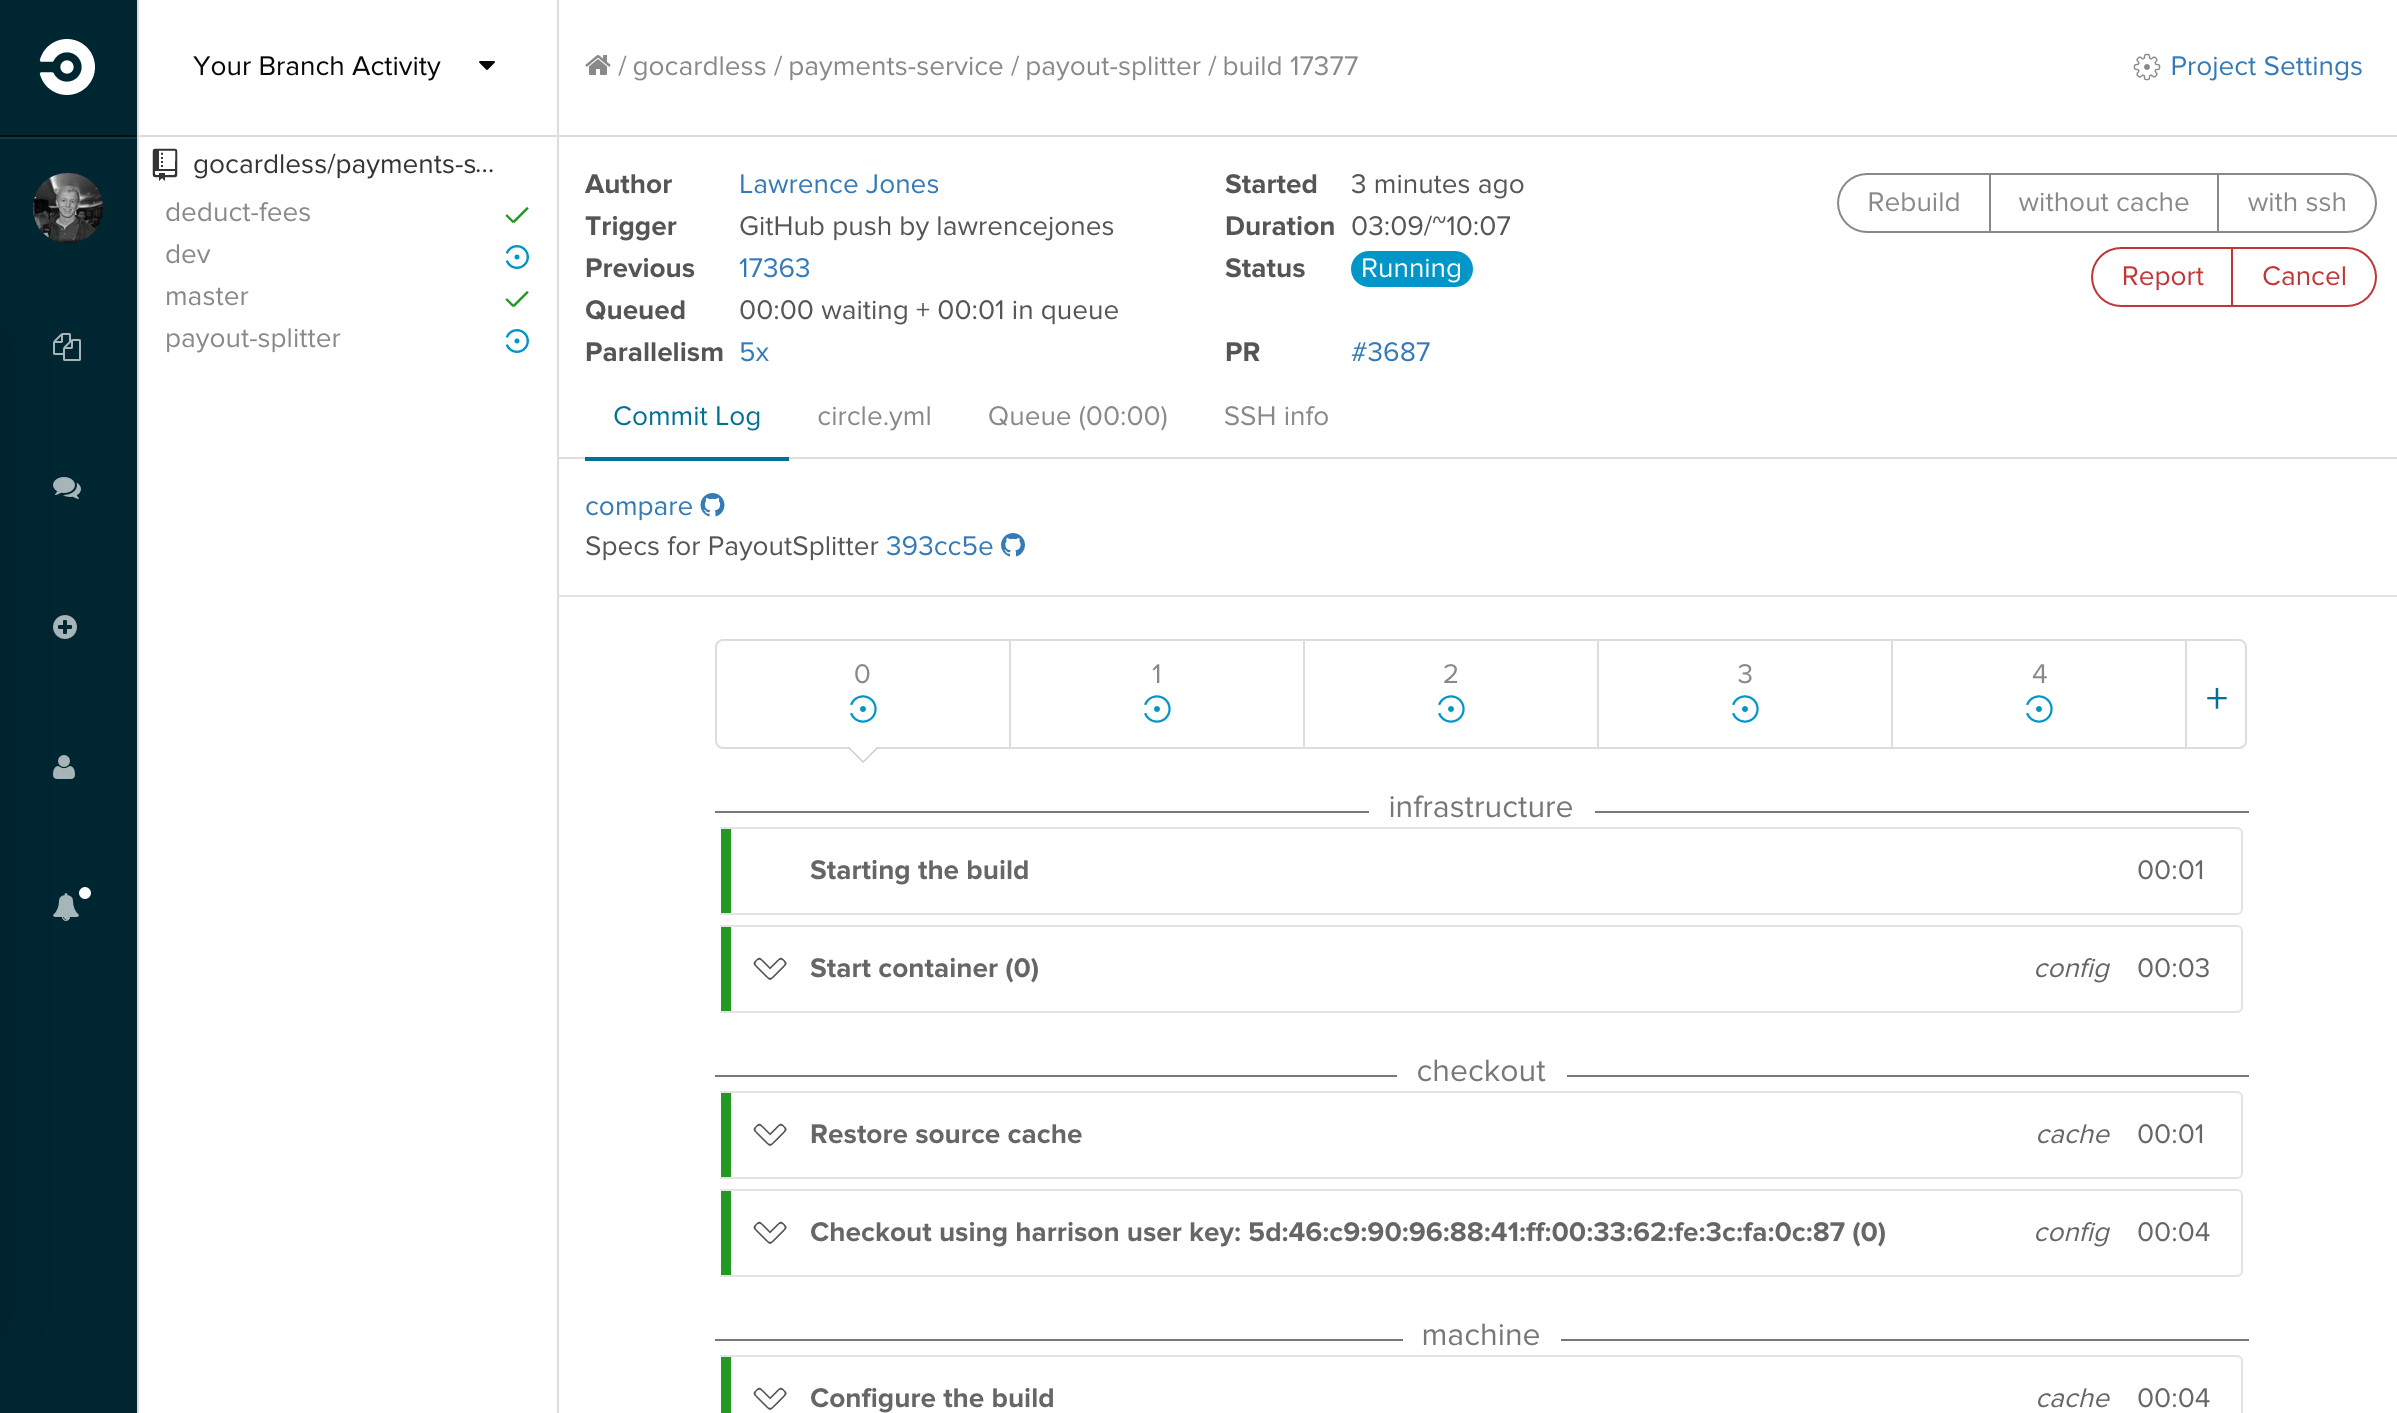
\includegraphics[width=1\textwidth]{lib/res/circle.png}
\caption{\label{fig:circle}\textit{\texttt{payments-service} tests on CircleCI
with 5 workers}}
\end{figure}

Stripe is an excellent case study on how this scales. Built on Rails, just as
GoCardless, Stripe have achieved 3m build times from this parallelisation, by
creating a test runner framework that \texttt{fork}s extensively on a high
powered Amazon EC instance. Stripe's Nelson Elhage says\dots

\begin{displayquote}

  The decision to invest effort in our own testing infrastructure wasn't
  necessarily obvious: we could have continued to use a third-party solution.
  However, spending a comparatively small amount of effort allowed the rest of our
  engineering organization to move significantly faster—and with more confidence.
  I'm also optimistic this test runner will continue to scale with us and support
  our growth for several years to come.\\

  \textit{Nelson Elhage - Running 3hrs of Ruby tests in under
  3m~\cite{stripeDistributedTesting}}

\end{displayquote}

Clearly Stripe figured out how to make their `good tests' run fast, and have
confidence they will continue to do so in future.

\[*\]

The comparison of Amazon and GoCardless testing ethos highlights some major
differences in organisational structure. Amazon with their many services cannot
afford to special case each team nor, as their Frugality principle suggests,
would they want to. GoCardless as a start-up has more flexibility, and can
manage each project on its own basis. Indeed, specifying a general rule for
everyone when your company is only four years old is probably an unwise move.

Regardless of their differences in size and technical ethos, Amazon and
GoCardless both exhibit key qualities of highly effective companies. Both strive
for pragmatism in their development practises, and favour highly technical
dialogue that works hard to include non-technical staff in the discussion.

Each follow Agile principles, but do so on their own terms. It's highly unusual
to find either adopting a procedure without questioning the value \textbf{within
the context of their own business}, which can be refreshing in an industry that
enjoys talking in absolutes.

%----------------------------------------------------------------------------------------
%   BIBLIOGRAPHY
%----------------------------------------------------------------------------------------

\medskip
\bibliography{lib/refs}{}
\bibliographystyle{plain}
\newpage

\end{document}
